% Provenance (never printed): see sources/outline_sources.md (Year 1: vertical structure of
% the atmosphere, lapse rates, potential temperature and static stability; the layered
% ocean, the equation of state of seawater, T-S diagrams and water masses). Exercise and
% problem values in the Book 3 scratch calculator calc/ch26.py; figures from
% figdata/bachelor-1/atmosphere_profile.py (U.S. Standard Atmosphere 1976) and
% seawater_eos.py (EOS-80 and the UNESCO 44 algorithms; WOA23 columns, datasets
% bachelor-1-woa23-* and Book 2's grade-10-woa23-arctic-*).
% Physics owns the hydrostatic relation, the isothermal atmosphere and its scale height,
% the first law, Laplace's relation and Archimedes' thrust (recalled). Book 1 (g8) gave
% the layers and the environmental lapse rate of 6.5 K/km; Book 2 (g10) the dry adiabatic
% rate admitted, stable and unstable air, the mixed layer, thermocline, halocline and
% pycnocline: re-founded here with derivations. The moist adiabat is the Year 2 volume's.
\chapter{La structure de l'atmosphère et de l'océan}\label{ch:b1:fluid-envelopes-structure}

Deux fois par jour, dans des stations météorologiques du monde entier, un ballon est lâché portant
une radiosonde, un petit instrument qui renvoie par radio la pression, la température
et l'humidité de l'air pendant qu'il monte~; il s'élève d'environ \qty{300}{m} par minute
et peut dépasser \qty{35}{km} avant que le ballon n'éclate. Loin en mer, un navire de
recherche descend au bout d'un câble vers l'abysse un bâti d'instruments et de bouteilles d'eau,
en mesurant la conductivité, la température et la profondeur tout du long. Les deux
profils, un de l'air et un de l'eau, sont la matière première de ce
chapitre. Les deux enveloppes sont stratifiées, et dans les deux la stratification est fixée par la masse volumique~:
fluide léger au-dessus du fluide lourd. Ce qui rend une couche légère ou lourde est moins évident
qu'il n'y paraît. Un air plus froid que l'air en dessous peut encore être le plus léger~;
une eau plus chaude que l'eau au-dessus peut encore être la plus lourde. Le
chapitre construit les deux outils qui démêlent cela, la \omterm{def:b1:fluid-envelopes-structure:potential-temperature}{température potentielle} et
l'\omterm{def:b1:fluid-envelopes-structure:eos}{équation d'état de l'eau de mer}.
% ledger: nws:radiosonde, nws:radiosonde-def, commons:ctd-rosette

\begin{omfigure}
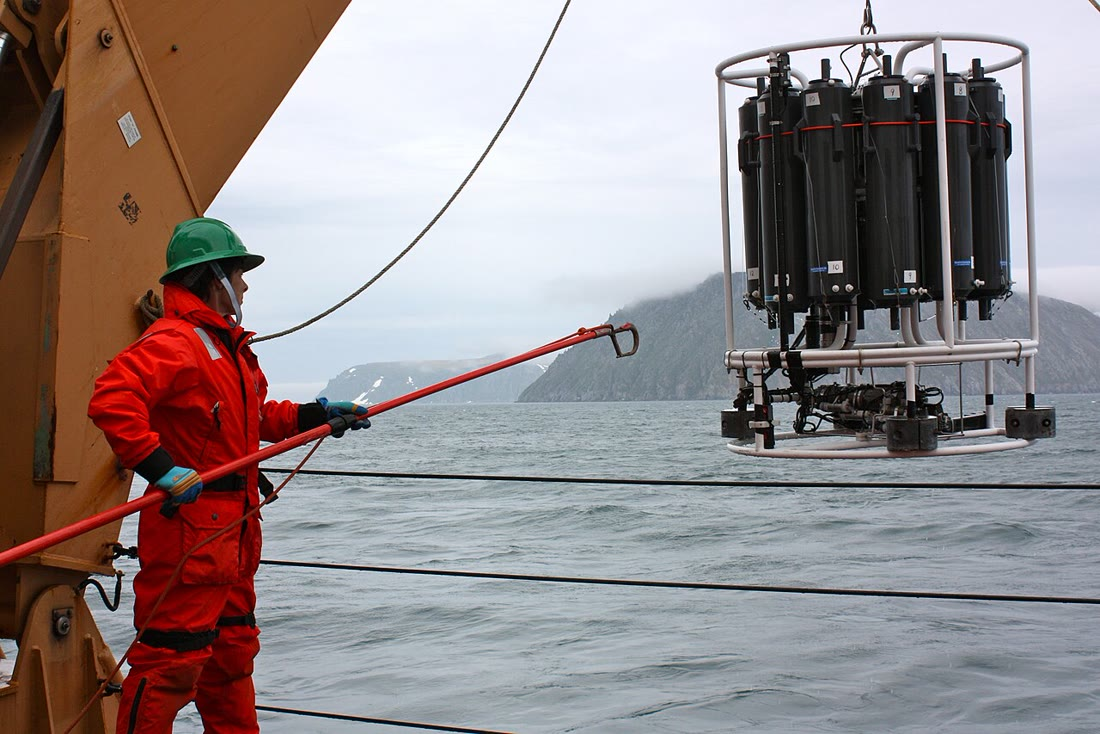
\includegraphics[width=0.62\linewidth]{images/book3/b1-ctd-rosette.jpg}

{\small Un CTD et sa rosette remontés à bord dans le détroit de Béring en
juin 2011. Les bouteilles grises autour du bâti sont fermées à des profondeurs choisies
pendant la remontée pour échantillonner l'eau~; les instruments au bas du bâti mesurent
la conductivité (dont on calcule la salinité), la température et la profondeur (en fait la
pression) en continu pendant la descente du bâti. (NASA Goddard Space Flight
Center, domaine public, via Wikimedia Commons.)}
\label{fig:b1:fluid-envelopes-structure:ctd}
\end{omfigure}
% ledger: commons:ctd-rosette, unesco44:atg-theta

\begin{recall}
Les volumes de physique donnent la relation hydrostatique, $\mathrm dp/\mathrm dz =
-\rho g$, pour un fluide au repos~; pour un gaz parfait de masse molaire $M$, $p = \rho R
T/M$, et dans une atmosphère isotherme la pression décroît comme $e^{-z/H}$ avec la
hauteur d'échelle $H = RT/(Mg)$. Ils énoncent le premier principe pour un système fermé et,
pour un gaz parfait, la relation de Laplace le long d'une transformation adiabatique
réversible, $pV^{\gamma} = $ constante, avec $\gamma = c_p/c_v$ et $c_p - c_v
= R/M$ par unité de masse. Un corps immergé dans un fluide reçoit une poussée vers le haut égale
au poids du fluide qu'il déplace (Archimède). Le livre~1 a nommé les couches de
l'atmosphère et le \omterm{def:b1:fluid-envelopes-structure:lapse-rate}{gradient vertical de température} de l'\omterm{def:b1:fluid-envelopes-structure:standard-atmosphere}{atmosphère standard},
\qty{6.5}{\celsius} par kilomètre dans la troposphère~; le livre~2 a admis le \omterm{def:b1:fluid-envelopes-structure:lapse-rate}{gradient
adiabatique sec}, \qty{9.8}{\celsius} par kilomètre, a qualifié l'air de stable ou d'instable
selon le sort d'une parcelle poussée vers le haut, et a décrit la \omterm{def:b1:fluid-envelopes-structure:ocean-layers}{couche de mélange},
la \omterm{def:b1:fluid-envelopes-structure:ocean-layers}{thermocline}, l'\omterm{def:b1:fluid-envelopes-structure:ocean-layers}{halocline} et la \omterm{def:b1:fluid-envelopes-structure:ocean-layers}{pycnocline} de l'océan. La salinité de l'eau
de mer est voisine de 35 grammes de sels dissous par kilogramme.
% ledger: ussa76:layers, nws:dalr, nos:salinity
\end{recall}

\section{La structure verticale de l'atmosphère}\label{sec:b1:fluid-envelopes-structure:atmosphere}

Deux sondages réels ne sont jamais identiques. Pour les comparer, un profil de référence
est fixé par convention.

\begin{definition}[Atmosphère standard]\label{def:b1:fluid-envelopes-structure:standard-atmosphere}
Une \emph{atmosphère standard}\index{atmosphere standard@atmosphère standard} est un profil de
température, de pression et de masse volumique en fonction de la hauteur fixé par convention~: air sec
de masse molaire constante, gaz parfait en équilibre hydrostatique, avec des valeurs données au
niveau de la mer et une température qui varie linéairement avec la hauteur dans des
couches successives. L'atmosphère standard de 1976 prend \qty{288.15}{K} et
\qty{101325}{Pa} au niveau de la mer, $M_0 = \qty{28.9644}{kg.kmol^{-1}}$,
$R^* = \qty{8314.32}{J.kmol^{-1}.K^{-1}}$ et $g_0 = \qty{9.80665}{m.s^{-2}}$.
\end{definition}
% ledger: ussa76:sea-level

Sous \qty{47}{km} le standard de 1976 a quatre couches
(\cref{tab:b1:fluid-envelopes-structure:layers}). La plus basse, la troposphère,
se refroidit de \qty{6.5}{K} par kilomètre~; à partir de son sommet, la tropopause, la
température reste à \qty{216.65}{K} pendant neuf kilomètres, puis monte. Les
hauteurs du standard sont des hauteurs géopotentielles, les hauteurs qu'une
pesanteur constante $g_0$ donnerait pour la même énergie potentielle~; sous \qty{32}{km} elles
diffèrent des hauteurs géométriques de moins de \qty{0.6}{\percent}
(\qty{11}{km} du standard se trouvent à \qty{11.02}{km}).
% ledger: ussa76:layers, ussa76:sea-level

\begin{table}[ht]
\centering
\small
\renewcommand{\arraystretch}{1.2}
\begin{tabular}{|l|c|c|c|c|}
\hline
Couche & Base (km) & $\mathrm dT/\mathrm dz$ (K/km) & $T$ à la base (K) & $p$ à la base (hPa) \\
\hline
1 (troposphère) & 0 & $-6.5$ & 288.15 & 1013.25 \\
2 (stratosphère) & 11 & 0.0 & 216.65 & 226.32 \\
3 (stratosphère) & 20 & $+1.0$ & 216.65 & 54.75 \\
4 (stratosphère) & 32 & $+2.8$ & 228.65 & 8.68 \\
\hline
\end{tabular}
\caption{Les quatre couches les plus basses de l'\omterm{def:b1:fluid-envelopes-structure:standard-atmosphere}{atmosphère standard} de 1976. Les gradients
et les valeurs au niveau de la mer sont des valeurs de définition~; les températures et pressions à
la base en sont calculées avec la \cref{prop:b1:fluid-envelopes-structure:layer-pressure}.}
\label{tab:b1:fluid-envelopes-structure:layers}
\end{table}
% ledger: ussa76:layers, ussa76:sea-level (bases computed in figdata/bachelor-1/atmosphere_profile.py)

Dans chaque couche la température est une fonction linéaire de la hauteur, si bien que la
relation hydrostatique peut s'intégrer sous forme close.

\begin{proposition}[Pression dans une couche à gradient constant]\label{prop:b1:fluid-envelopes-structure:layer-pressure}
Dans une couche d'air sec où $T = T_b - L\,(z - z_b)$ avec $L \neq 0$ constant, la
pression est
\[
  p = p_b \left(\frac{T}{T_b}\right)^{gM/(RL)},
\]
où $T_b$ et $p_b$ sont les valeurs à la base $z_b$. Quand $L = 0$ la
pression décroît exponentiellement avec la hauteur d'échelle $H = RT_b/(Mg)$.
\end{proposition}

\begin{proof}
La relation hydrostatique et le gaz parfait donnent $\mathrm dp/p = -(gM/R)\,\mathrm
dz/T$. Comme $\mathrm dT = -L\,\mathrm dz$, cela fait $\mathrm dp/p =
(gM/(RL))\,\mathrm dT/T$, qui s'intègre en $\ln(p/p_b) = (gM/(RL))
\ln(T/T_b)$. Pour $L = 0$, $T = T_b$ et $\ln(p/p_b) = -(z - z_b)/H$~:
l'atmosphère isotherme des volumes de physique.
\end{proof}

Dans la troposphère du standard, $gM/(RL) = 9.80665 \times 28.9644 /
(8314.32 \times 0.0065) = 5.256$, et à \qty{11}{km}, $T = 216.65$~K~:
$p = \num{101325} \times (216.65/288.15)^{5.256} = \qty{22632}{Pa}$, un peu
moins du quart de la valeur au niveau de la mer. Dans la couche isotherme au-dessus, $H =
8314.32 \times 216.65/(28.9644 \times 9.80665) = \qty{6.34}{km}$, et neuf
kilomètres plus haut la pression a encore chuté d'un facteur $e^{9/6.34} =
4.13$, jusqu'à \qty{5475}{Pa}. Puisque la pression à un niveau est le poids, par unité
d'aire, de l'air au-dessus, la moitié de la masse de l'\omterm{def:b1:fluid-envelopes-structure:standard-atmosphere}{atmosphère standard} se trouve sous
\qty{5.5}{km} et les neuf dixièmes sous \qty{16}{km}.
% ledger: ussa76:sea-level, ussa76:layers (values computed in figdata/bachelor-1/atmosphere_profile.py)

\section{Gradients verticaux et température potentielle}\label{sec:b1:fluid-envelopes-structure:lapse}

\begin{definition}[Gradient vertical de l'environnement et gradient adiabatique sec]\label{def:b1:fluid-envelopes-structure:lapse-rate}
Le \emph{gradient vertical de température de l'environnement}\index{gradient vertical de temperature@gradient vertical de température} est $\Gamma =
-\mathrm dT/\mathrm dz$, le taux auquel la température de l'air au repos
décroît avec la hauteur, tel qu'un sondage le mesure. Le \emph{gradient adiabatique
sec}\index{gradient adiabatique sec} $\Gamma_d$ est le taux auquel la
température d'une \omterm{def:b1:fluid-envelopes-structure:parcel}{parcelle d'air} non saturé décroît quand la parcelle est soulevée.
\end{definition}
% ledger: nws:dalr

Un gradient est positif quand la température décroît avec la hauteur. Les deux taux
sont de natures différentes~: le premier décrit l'état de l'atmosphère à un
instant~; le second, la transformation d'un morceau d'air qui se déplace.

\begin{definition}[Parcelle d'air]\label{def:b1:fluid-envelopes-structure:parcel}
Une \emph{parcelle d'air}\index{parcelle d'air} est un volume d'air suivi dans son
mouvement, assez petit pour avoir une seule température et une seule pression et ne pas
perturber l'air alentour, assez grand pour garder son identité~: il n'échange ni
masse ni, pendant un déplacement rapide, chaleur avec son environnement, et sa
pression est à chaque instant celle de l'air environnant.
\end{definition}

La parcelle est une idéalisation, comme le système fermé de la thermodynamique~: les
résultats ci-dessous valent pour l'air réel dans la mesure où un morceau d'air en mouvement échange
peu de chaleur et peu de masse avec son environnement.

\begin{theorem}[Le gradient adiabatique sec]\label{thm:b1:fluid-envelopes-structure:dry-adiabatic}
Une \omterm{def:b1:fluid-envelopes-structure:parcel}{parcelle d'air} sec, soulevée de façon adiabatique et réversible à travers un air au repos de
température presque identique, se refroidit au taux
\[
  \Gamma_d = \frac{g}{c_p},
\]
où $c_p$ est la capacité thermique massique de l'air à pression constante. Avec $c_p =
\qty{1004.7}{J.kg^{-1}.K^{-1}}$, $\Gamma_d = \qty{9.76}{K.km^{-1}}$.
\end{theorem}

\begin{proof}
Pour un kilogramme de la parcelle, de température $T_p$ et de masse volumique $\rho_p$, le
premier principe d'une transformation réversible sans échange de chaleur, écrit avec
l'enthalpie, est $c_p\,\mathrm dT_p - \mathrm dp/\rho_p = 0$. La pression de la
parcelle est celle de l'air alentour, qui est hydrostatique~: $\mathrm dp = -\rho_e
g\,\mathrm dz$, avec $\rho_e$ la masse volumique de l'air environnant. D'où
\[
  \frac{\mathrm dT_p}{\mathrm dz} = -\frac{g}{c_p}\,\frac{\rho_e}{\rho_p}
  = -\frac{g}{c_p}\,\frac{T_p}{T_e},
\]
puisqu'à pression égale les masses volumiques de deux gaz parfaits de même masse molaire
sont dans le rapport inverse de leurs températures. Quand la parcelle est à peu près à la
température de son environnement, $T_p/T_e \approx 1$ et $-\mathrm dT_p/\mathrm dz
= g/c_p$. Pour l'air sec, gaz parfait diatomique, $\gamma = 1.4$, donc $c_p =
\gamma/(\gamma - 1) \times R/M = 3.5 \times 8314.32/28.9644 =
\qty{1004.7}{J.kg^{-1}.K^{-1}}$, et $\Gamma_d = 9.80665/1004.7 =
\qty{0.00976}{K.m^{-1}}$.
\end{proof}
% ledger: nasa:grc-gamma, ussa76:sea-level, nws:dalr

Une parcelle de \qty{10}{K} plus chaude que son environnement, vers \qty{280}{K}, se refroidit de
$\Gamma_d \times 290/280$, soit \qty{3.6}{\percent} plus vite~; la correction est
négligée dans la suite. Le taux ne dépend ni de la pression ni de la
température de la parcelle, et une parcelle qui descend se réchauffe au même taux, comme
le livre~2 l'a suivi pour l'air passant une montagne.

L'intégration de la même équation sans l'étape hydrostatique donne une grandeur que
la parcelle emporte avec elle.

\begin{proposition}[Température potentielle]\label{prop:b1:fluid-envelopes-structure:theta}
Le long d'une transformation adiabatique réversible d'air sec,
\[
  \theta = T\left(\frac{p_0}{p}\right)^{\kappa},\qquad \kappa = \frac{R}{Mc_p} =
  \frac{\gamma - 1}{\gamma} = \frac{2}{7},
\]
reste constante, quelle que soit la pression de référence $p_0$.
\end{proposition}

\begin{proof}
À partir de $c_p\,\mathrm dT = \mathrm dp/\rho$ et $\rho = pM/(RT)$, $c_p\,\mathrm dT/T
= (R/M)\,\mathrm dp/p$, donc $\ln T - \kappa \ln p$ est constant, et $T
p^{-\kappa}$ aussi~; la multiplication par la constante $p_0^{\kappa}$ donne $\theta$. C'est
la relation de Laplace écrite avec $T$ et $p$.
\end{proof}

\begin{definition}[Température potentielle]\label{def:b1:fluid-envelopes-structure:potential-temperature}
La \emph{température potentielle}\index{temperature potentielle@température potentielle} $\theta$ d'une
\omterm{def:b1:fluid-envelopes-structure:parcel}{parcelle d'air} sec est la température qu'elle aurait si elle était amenée adiabatiquement à
la pression de référence $p_0 = \qty{1000}{hPa}$~: $\theta = T\,(1000/p)^{2/7}$ avec
$p$ en hectopascals et $T$ en kelvins.
\end{definition}
% ledger: nws:potential-temperature

La \omterm{def:b1:fluid-envelopes-structure:potential-temperature}{température potentielle} est une étiquette qu'une parcelle sèche garde quand elle monte ou
descend sans échanger de chaleur, comme la salinité d'une parcelle d'eau. Le chauffage par
rayonnement, par condensation de l'eau ou par mélange la modifie~; le reste, non.

\begin{example}[La tropopause de l'atmosphère standard]\label{ex:b1:fluid-envelopes-structure:tropopause}
À la surface du standard, $\theta = 288.15 \times (1000/1013.25)^{2/7} =
\qty{287.07}{K}$. À la tropopause, $T = \qty{216.65}{K}$ et $p =
\qty{226.32}{hPa}$~: $\theta = 216.65 \times (1000/226.32)^{2/7} = 216.65 \times
1.529 = \qty{331.2}{K}$. De l'air de la tropopause ramené adiabatiquement à
\qty{1000}{hPa} arriverait à \qty{331.2}{K}, \qty{44}{K} plus chaud que de l'air de surface
ramené à la même pression. La température chute de \qty{71.5}{K} du
sol à la tropopause, et pourtant la \omterm{def:b1:fluid-envelopes-structure:potential-temperature}{température potentielle} croît de
\qty{44}{K}.
\end{example}
% ledger: ussa76:layers, nws:potential-temperature (values computed in figdata/bachelor-1/atmosphere_profile.py)

\section{La stabilité statique}\label{sec:b1:fluid-envelopes-structure:stability}

\begin{definition}[Stabilité statique~; inversion de température]\label{def:b1:fluid-envelopes-structure:stability}
La \emph{stabilité statique}\index{stabilite statique@stabilité statique} d'une couche au repos est sa
réponse à un petit déplacement vertical d'une parcelle. La couche a une
\emph{stratification stable}\index{stratification stable} si la parcelle déplacée
est repoussée vers son niveau, une \emph{stratification
instable}\index{stratification instable} si elle est repoussée plus loin,
et une \emph{stratification neutre}\index{stratification neutre} si aucune force
ne s'exerce sur elle. Une \emph{inversion de température}\index{inversion de temperature@inversion de température} est une
couche dans laquelle la température croît avec la hauteur.
\end{definition}
% ledger: nws:inversion

\begin{theorem}[Le critère de stabilité statique]\label{thm:b1:fluid-envelopes-structure:stability}
Une couche d'air sec au repos, de température $T$ et de gradient vertical de l'environnement
$\Gamma$, est stable si $\Gamma < \Gamma_d$, neutre si $\Gamma = \Gamma_d$ et
instable si $\Gamma > \Gamma_d$~; de façon équivalente, elle est stable si et seulement si sa
\omterm{def:b1:fluid-envelopes-structure:potential-temperature}{température potentielle} croît avec la hauteur. Une parcelle déplacée d'un petit
$\delta z$ dans une couche stable oscille autour de son niveau à la
pulsation $N$, où
\[
  N^2 = \frac{g}{T}\,(\Gamma_d - \Gamma) = \frac{g}{\theta}\,\frac{\mathrm d\theta}{\mathrm dz}.
\]
\end{theorem}

\begin{proof}
Une parcelle à la température $T$ de son niveau est soulevée de $\delta z$. Elle arrive
à $T - \Gamma_d\,\delta z$, tandis que l'air alentour est à $T - \Gamma\,\delta z$.
Par unité de masse, la parcelle subit son poids et la poussée d'Archimède, une
accélération nette vers le haut $g\,(\rho_e - \rho_p)/\rho_p = g\,(T_p - T_e)/T_e$, les
pressions étant égales. Au premier ordre en $\delta z$ cela fait
\[
  \frac{\mathrm d^2 \delta z}{\mathrm dt^2} = -\frac{g}{T}\,(\Gamma_d - \Gamma)\,\delta z = -N^2\,\delta z .
\]
Si $\Gamma < \Gamma_d$, $N^2 > 0$ et la parcelle oscille à la
pulsation $N$~; si $\Gamma > \Gamma_d$ le déplacement croît exponentiellement~; si
$\Gamma = \Gamma_d$ aucune force ne s'exerce. Pour la seconde forme, prenons la
dérivée logarithmique de $\theta = T (p_0/p)^{\kappa}$ et utilisons la relation hydrostatique~:
\[
  \frac{1}{\theta}\frac{\mathrm d\theta}{\mathrm dz} = \frac{1}{T}\frac{\mathrm dT}{\mathrm dz}
  - \frac{\kappa}{p}\frac{\mathrm dp}{\mathrm dz} = -\frac{\Gamma}{T} + \frac{\kappa\,\rho g}{p}
  = -\frac{\Gamma}{T} + \frac{\kappa g M}{RT} = \frac{\Gamma_d - \Gamma}{T},
\]
puisque $\kappa M/R = 1/c_p$.
\end{proof}

La pulsation $N$ s'appelle la fréquence de flottabilité. Dans la troposphère
du standard, près du sol, $N^2 = (9.80665/288.15) \times (9.761 -
6.5)\times10^{-3} = \qty{1.11e-4}{s^{-2}}$, $N = \qty{0.0105}{s^{-1}}$, et la
période $2\pi/N$ de l'oscillation est d'environ \qty{10}{min}. Dans la basse
stratosphère isotherme $\Gamma = 0$~: $N = \qty{0.0210}{s^{-1}}$, deux fois plus grand, une
période de cinq minutes. La stratosphère est un couvercle~: elle résiste au mouvement vertical
bien plus fortement que la troposphère en dessous d'elle.
% ledger: ussa76:layers (values computed in figdata/bachelor-1/atmosphere_profile.py)

\begin{omfigure}
\begin{tikzpicture}
\begin{axis}[name=tz, omrecord, width=0.46\linewidth, height=7.2cm, xmin=160, xmax=300,
  ymin=0, ymax=32, xlabel={température (K)}, ylabel={hauteur (km)}, xtick={160,200,...,300},
  ytick={0,5,...,30}]
% figdata/bachelor-1/atmosphere_profile.py; ledger: ussa76:sea-level, ussa76:layers, nasa:grc-gamma
\addplot[omDef, line width=0.9pt] table[x=T_K, y=z_km] {figdata/out/bachelor-1-atmosphere_profile-profile.dat};
\addplot[omThm, dashed, line width=0.7pt] table[x=T_K, y=z_km] {figdata/out/bachelor-1-atmosphere_profile-adiabat.dat};
\addplot[only marks, mark=*, mark size=1.6pt, black] table[x=T_K, y=z_km] {figdata/out/bachelor-1-atmosphere_profile-tropo.dat};
\node[font=\scriptsize, text=omThm, anchor=west, align=left] at (axis cs:163,17.0) {adiabatique sèche\\depuis la surface};
\node[font=\scriptsize, text=omDef, anchor=west] at (axis cs:252,6.4) {standard};
\node[font=\scriptsize, anchor=east] at (axis cs:214.5,11.9) {tropopause};
\end{axis}
\begin{axis}[at={(tz.east)}, anchor=west, xshift=1.3cm, omrecord, width=0.46\linewidth, height=7.2cm,
  xmin=250, xmax=900, ymin=0, ymax=32, xlabel={température potentielle (K)}, ylabel={hauteur (km)},
  xtick={300,500,700,900}, ytick={0,5,...,30}]
\addplot[omDef, line width=0.9pt] table[x=theta_K, y=z_km] {figdata/out/bachelor-1-atmosphere_profile-profile.dat};
\addplot[only marks, mark=*, mark size=1.6pt, black] table[x=theta_K, y=z_km] {figdata/out/bachelor-1-atmosphere_profile-tropo.dat};
\node[font=\scriptsize, anchor=west] at (axis cs:345,10.2) {\num{331} K};
\end{axis}
\end{tikzpicture}

{\small L'\omterm{def:b1:fluid-envelopes-structure:standard-atmosphere}{atmosphère standard} de 1976 jusqu'à \qty{32}{km}. À gauche~: la température, avec
l'adiabatique sèche qu'une parcelle soulevée de la surface suivrait (tirets). Le
standard se refroidit plus lentement que l'adiabatique, donc il est stable partout. À droite~:
la \omterm{def:b1:fluid-envelopes-structure:potential-temperature}{température potentielle}, qui croît avec la hauteur partout, doucement dans la
troposphère et fortement au-dessus de la tropopause (point).}
\label{fig:b1:fluid-envelopes-structure:theta}
\end{omfigure}
% ledger: ussa76:sea-level, ussa76:layers, nasa:grc-gamma, nws:potential-temperature

Sur un diagramme de la température en fonction de la hauteur, le critère compare deux pentes
(figure ci-dessous)~: la parcelle suit l'adiabatique sèche passant par son point de départ,
et la question est de savoir de quel côté du sondage elle se retrouve après un petit
déplacement.

\begin{omfigure}
\begin{tikzpicture}[x=0.55cm, y=0.55cm, >={Stealth[length=2mm]}]
\foreach \dx/\envtop/\verdict in {0/-0.8/{couche stable~: la parcelle retombe}, 9/-3.8/{couche instable~: la parcelle continue de monter}} {
  \begin{scope}[xshift=\dx cm]
  \draw[->] (0,0) -- (7.2,0) node[below left, font=\scriptsize] {température};
  \draw[->] (0,0) -- (0,6.4) node[above right, font=\scriptsize] {hauteur};
  % sounding (environment): solid; dry adiabat through the starting point P: dashed
  \draw[omDef, line width=0.9pt] (5.0,0.6) -- (5.0+\envtop,5.4);
  \draw[omThm, dashed, line width=0.8pt] (5.0,0.6) -- (2.6,5.4);
  \fill (5.0,0.6) circle (2pt) node[right, font=\scriptsize] {$P$};
  \draw[densely dotted] (0,4.2) node[left, font=\scriptsize] {$z + \delta z$} -- (7,4.2);
  \fill[omThm] (3.2,4.2) circle (1.8pt);
  \fill[omDef] ({5.0+\envtop*3.6/4.8},4.2) circle (1.8pt);
  \node[font=\scriptsize, anchor=north] at (3.6,-0.5) {\verdict};
  \end{scope}
}
\end{tikzpicture}

{\small La méthode de la parcelle. Trait plein bleu~: le sondage~; tirets rouges~:
l'adiabatique sèche passant par $P$. Une parcelle part de $P$ à la température de l'air autour
d'elle et est soulevée jusqu'à $z + \delta z$ le long de l'adiabatique sèche (point rouge)~; le sondage
donne la température de l'air en ce lieu (point bleu). À gauche~: le sondage
se refroidit plus lentement que l'adiabatique~; la parcelle arrive plus froide, donc plus dense, que
son environnement et retombe. À droite~: le sondage se refroidit plus vite que
l'adiabatique~; la parcelle arrive plus chaude et continue de monter.}
\label{fig:b1:fluid-envelopes-structure:parcel}
\end{omfigure}

\begin{method}[Lire la stabilité d'un sondage]\label{met:b1:fluid-envelopes-structure:sounding}
\begin{enumerate}
  \item Diviser le sondage en couches entre les niveaux où la pente change.
  \item Dans chaque couche calculer $\Gamma = -(T_2 - T_1)/(z_2 - z_1)$, en kelvins par
        kilomètre.
  \item Comparer à $\Gamma_d = \qty{9.8}{K/km}$~: $\Gamma > \Gamma_d$ instable,
        $\Gamma$ proche de $\Gamma_d$ neutre, $\Gamma < \Gamma_d$ stable~; un
        $\Gamma$ négatif est une inversion, le cas le plus stable.
  \item Là où des pressions sont données plutôt que des hauteurs, calculer $\theta =
        T(1000/p)^{2/7}$ à chaque niveau~: $\theta$ décroissant vers le haut marque une
        couche instable, constant une couche neutre, croissant une couche stable.
\end{enumerate}
\end{method}

Une couche instable ne dure pas~: un déplacement dans elle croît exponentiellement, au
taux $\sqrt{-N^2}$, et les parcelles qu'elle libère la retournent, en la mélangeant jusqu'à ce que
sa \omterm{def:b1:fluid-envelopes-structure:potential-temperature}{température potentielle} soit uniforme et son gradient vertical vaille $\Gamma_d$. Une couche
chauffée par en dessous, par un sol chaud ou une mer chaude, est poussée vers l'instabilité~;
une couche refroidie par en dessous, vers la stabilité. Une inversion coiffe tout ce qui se trouve en
dessous d'elle~: une parcelle montant d'en dessous se retrouve plus froide que son environnement dès
qu'elle y entre. Au-dessus de \qty{20}{km} toute la stratosphère du standard est une
inversion.

Tout cela suppose de l'air sec. Une parcelle montante qui devient saturée libère
de la chaleur latente quand son eau se condense et se refroidit plus lentement que $\Gamma_d$~;
l'adiabatique saturée et l'instabilité conditionnelle qu'elle apporte sont l'objet du
volume de deuxième année.
% ledger: nws:inversion, nws:dalr

\section{L'océan stratifié}\label{sec:b1:fluid-envelopes-structure:ocean}

L'océan n'échange de la chaleur et de l'eau avec l'atmosphère qu'à sa surface,
par chauffage et refroidissement, évaporation et pluie. Sa structure verticale a
trois ingrédients, la température, la salinité et la masse volumique.

\begin{definition}[Couche de mélange, thermocline, halocline, pycnocline]\label{def:b1:fluid-envelopes-structure:ocean-layers}
La \emph{couche de mélange}\index{couche de melange@couche de mélange} est la couche de surface de l'océan
dont la température, la salinité et la masse volumique sont presque uniformes avec la profondeur~; sa
profondeur se lit sur un profil comme la profondeur où la température diffère d'abord
de sa valeur de surface d'un seuil choisi, souvent \qty{0.5}{\celsius}. La
\emph{thermocline}\index{thermocline}, l'\emph{halocline}\index{halocline} et
la \emph{pycnocline}\index{pycnocline} sont les couches en dessous d'elle où la
température, la salinité et la masse volumique respectivement changent le plus vite avec la
profondeur.
\end{definition}

La pression dans l'océan est donnée en décibars, parce qu'un décibar,
\qty{e4}{Pa}, est presque la pression d'un mètre d'eau de mer~: à
\qty{30}{\degree} de \omterm{def:b1:spherical-astronomy:geographic}{latitude}, \qty{1000}{dbar} se trouvent à \qty{990.8}{m} et
\qty{10000}{dbar} à \qty{9712.7}{m}.
% ledger: unesco:eos80-checks (DEPTH table computed in figdata/bachelor-1/seawater_eos.py)

L'eau est presque incompressible, mais pas tout à fait, et une parcelle d'eau remontée
des profondeurs se dilate et se refroidit un peu, comme une \omterm{def:b1:fluid-envelopes-structure:parcel}{parcelle d'air}. Le
gradient adiabatique de l'eau de mer est petit, environ \qty{0.04}{\celsius} par
\qty{1000}{dbar} en surface à \qty{0}{\celsius} et \qty{0.09}{\celsius}
par \qty{1000}{dbar} à \qty{3000}{dbar}, contre \num{9.8} par kilomètre dans
l'air~; mais sur cinq kilomètres cela s'additionne en quelques dixièmes de degré, plus que
les différences entre eaux profondes. Les océanographes comparent donc les eaux aussi par
leur température \emph{potentielle}~: la température qu'une parcelle aurait si elle était
remontée adiabatiquement, sans changement de salinité, jusqu'à la surface. Une eau de
\qty{2}{\celsius} à \qty{4000}{dbar} et de salinité 35 a une \omterm{def:b1:fluid-envelopes-structure:potential-temperature}{température
potentielle} de \qty{1.66}{\celsius}. Dans les niveaux les plus profonds de l'Atlantique
Sud à \qty{10.5}{\degree S}, la température mesurée passe de
\qty{0.730}{\celsius} à \qty{5400}{m} à \qty{0.731}{\celsius} à \qty{5500}{m}
tandis que la \omterm{def:b1:fluid-envelopes-structure:potential-temperature}{température potentielle} chute de \qty{0.261}{\celsius} à
\qty{0.250}{\celsius}~: le réchauffement est de la compression, non de la chaleur.
% ledger: unesco44:atg-theta, data:b3-woa23 (values computed in figdata/bachelor-1/seawater_eos.py)

\begin{omfigure}
\begin{tikzpicture}
\begin{groupplot}[group style={group size=3 by 1, horizontal sep=0.55cm, yticklabels at=edge left},
  omrecord, omdepth, width=0.365\linewidth, height=7.4cm, ymin=0, ymax=2000,
  ytick={0,500,1000,1500,2000}, y tick label style={/pgf/number format/.cd, set thousands separator={}},
  every axis label/.append style={font=\small}]
\nextgroupplot[xmin=-2, xmax=28, xlabel={$\theta$ (\si{\celsius})}, ylabel={profondeur (m)}, xtick={0,10,20}]
% figdata/bachelor-1/seawater_eos.py; WOA23 (datasets bachelor-1-woa23-*, grade-10-woa23-arctic-*); ledger: data:b3-woa23, data:b2-woa23, unesco44:atg-theta
\addplot[omThm, line width=0.8pt] table[x=theta, y=depth] {figdata/out/bachelor-1-seawater_eos-prof-sa10.dat};
\addplot[omProp, line width=0.8pt] table[x=theta, y=depth] {figdata/out/bachelor-1-seawater_eos-prof-sa30.dat};
\addplot[omDef, line width=0.8pt] table[x=theta, y=depth] {figdata/out/bachelor-1-seawater_eos-prof-arctic.dat};
\draw[omThm, line width=0.8pt] (axis cs:9,1250) -- (axis cs:13,1250) node[right, font=\scriptsize, text=black] {\qty{10.5}{\degree S}};
\draw[omProp, line width=0.8pt] (axis cs:9,1450) -- (axis cs:13,1450) node[right, font=\scriptsize, text=black] {\qty{30.5}{\degree S}};
\draw[omDef, line width=0.8pt] (axis cs:9,1650) -- (axis cs:13,1650) node[right, font=\scriptsize, text=black] {\qty{75.5}{\degree N}};
\nextgroupplot[xmin=28, xmax=37.5, xlabel={salinité}, xtick={28,31,34,37}]
\addplot[omThm, line width=0.8pt] table[x=s, y=depth] {figdata/out/bachelor-1-seawater_eos-prof-sa10.dat};
\addplot[omProp, line width=0.8pt] table[x=s, y=depth] {figdata/out/bachelor-1-seawater_eos-prof-sa30.dat};
\addplot[omDef, line width=0.8pt] table[x=s, y=depth] {figdata/out/bachelor-1-seawater_eos-prof-arctic.dat};
\nextgroupplot[xmin=22, xmax=28.5, xlabel={$\sigma_\theta$ (\si{kg.m^{-3}})}, xtick={22,24,26,28}]
\addplot[omThm, line width=0.8pt] table[x=sigma, y=depth] {figdata/out/bachelor-1-seawater_eos-prof-sa10.dat};
\addplot[omProp, line width=0.8pt] table[x=sigma, y=depth] {figdata/out/bachelor-1-seawater_eos-prof-sa30.dat};
\addplot[omDef, line width=0.8pt] table[x=sigma, y=depth] {figdata/out/bachelor-1-seawater_eos-prof-arctic.dat};
\end{groupplot}
\end{tikzpicture}

{\small \omterm{def:b1:fluid-envelopes-structure:potential-temperature}{Température potentielle}, salinité et \omterm{def:b1:fluid-envelopes-structure:eos}{anomalie de densité} potentielle
(\cref{def:b1:fluid-envelopes-structure:eos}) dans les \qty{2000}{m} supérieurs, en
moyenne annuelle, en trois lieux~: l'Atlantique Sud tropical (\qty{10.5}{\degree
S}, \qty{25.5}{\degree O}), l'Atlantique Sud subtropical (\qty{30.5}{\degree
S}, \qty{25.5}{\degree O}) et le bassin Canada de l'océan Arctique
(\qty{75.5}{\degree N}, \qty{150.5}{\degree O}). Données~: World Ocean Atlas 2023.}
\label{fig:b1:fluid-envelopes-structure:profiles}
\end{omfigure}
% ledger: data:b3-woa23, data:b2-woa23, unesco:eos80, unesco44:atg-theta

Les trois colonnes de la figure ci-dessus montrent les trois sortes d'océan supérieur. Sous
les tropiques, une \omterm{def:b1:fluid-envelopes-structure:ocean-layers}{couche de mélange} chaude vers \qty{26.5}{\celsius} repose sur une \omterm{def:b1:fluid-envelopes-structure:ocean-layers}{thermocline}
marquée~: entre \qty{100}{m} et \qty{200}{m} la \omterm{def:b1:fluid-envelopes-structure:potential-temperature}{température potentielle}
chute de \qty{24.0}{\celsius} à \qty{14.4}{\celsius}, et la masse volumique la suit,
si bien que la \omterm{def:b1:fluid-envelopes-structure:ocean-layers}{thermocline} est aussi la \omterm{def:b1:fluid-envelopes-structure:ocean-layers}{pycnocline}. À \qty{30.5}{\degree S} la
surface est plus fraîche, \qty{21.1}{\celsius}, et la chute plus graduelle, répartie sur
les \qty{800}{m} supérieurs. Dans les deux, la salinité est la plus élevée près de la surface et
décroît vers le bas~; elle s'oppose à la stratification, ce que la température
compense largement. La colonne arctique
est le cas inverse. Son eau de surface, à \qty{-1.4}{\celsius}, est la plus froide
des trois, et pourtant la plus légère, $\sigma_\theta = 22.5$, parce que sa salinité n'est
que de \num{28.1}~; la salinité monte à \num{34.5} à \qty{300}{m}. L'\omterm{def:b1:fluid-envelopes-structure:ocean-layers}{halocline} est
la \omterm{def:b1:fluid-envelopes-structure:ocean-layers}{pycnocline} ici. En dessous se trouve une couche plus chaude que l'eau au-dessus, près de
\qty{0.7}{\celsius} à \qty{475}{m}~: une \omterm{def:b1:fluid-envelopes-structure:stability}{inversion de température} parfaitement
stable, maintenue en bas par son sel.
% ledger: data:b3-woa23, data:b2-woa23 (values computed in figdata/bachelor-1/seawater_eos.py)

\section{La masse volumique de l'eau de mer et les diagrammes T--S}\label{sec:b1:fluid-envelopes-structure:ts}

\begin{definition}[Équation d'état de l'eau de mer~; coefficient de contraction haline~; anomalie de densité]\label{def:b1:fluid-envelopes-structure:eos}
L'\emph{équation d'état de l'eau de mer}\index{equation d'etat de l'eau de mer@équation d'état de l'eau de mer}
donne sa masse volumique $\rho(S, T, p)$ en fonction de la salinité, de la température et de la
pression. Le \emph{coefficient de contraction haline}\index{coefficient de contraction haline} est $\beta = (1/\rho)\,\partial\rho/\partial S$ à température et pression
constantes. L'\emph{anomalie de densité}\index{anomalie de densite@anomalie de densité}
$\sigma$ est une masse volumique moins \qty{1000}{kg.m^{-3}}~: $\sigma_t = \rho(S, T, 0) -
1000$ emploie la température mesurée à pression marine nulle, et l'anomalie
de densité potentielle $\sigma_\theta = \rho(S, \theta, 0) - 1000$ la \omterm{def:b1:fluid-envelopes-structure:potential-temperature}{température
potentielle}.
\end{definition}
% ledger: teos10:alpha-beta, teos10:sigma

L'équation d'état n'est pas déduite de premiers principes mais ajustée sur des
mesures de laboratoire. L'équation internationale de 1980 à la pression de
la surface est un polynôme à quinze coefficients, $\rho = \rho_w(T) +
A(T)\,S + B(T)\,S^{3/2} + C\,S^2$, où $\rho_w$ est la masse volumique de l'eau pure~;
elle donne $\rho(35, \qty{0}{\celsius}) = \qty{1028.1063}{kg.m^{-3}}$. Une
description thermodynamique de l'eau de mer, TEOS-10, a été adoptée en 2009 pour la remplacer
comme description officielle~; l'équation de 1980 est employée ici parce que son polynôme
tient sur une page. Son coefficient de dilatation
thermique $\alpha = -(1/\rho)\,\partial\rho/\partial T$ est le
coefficient des volumes de physique.
% ledger: unesco:eos80, teos10:alpha-beta, teos10:replaced

\begin{table}[ht]
\centering
\small
\renewcommand{\arraystretch}{1.2}
\begin{tabular}{|c|c|c|c|}
\hline
$T$ (\si{\celsius}) & $\rho(35, T, 0)$ (\si{kg.m^{-3}}) & $\alpha$ (\si{K^{-1}}) & $\beta$ \\
\hline
0 & 1028.106 & \num{0.53e-4} & \num{7.85e-4} \\
10 & 1026.952 & \num{1.67e-4} & \num{7.61e-4} \\
25 & 1023.343 & \num{2.97e-4} & \num{7.39e-4} \\
\hline
\end{tabular}
\caption{Masse volumique et coefficients de dilatation de l'eau de mer de salinité 35 à la
pression de surface, d'après l'équation d'état internationale de 1980.}
\label{tab:b1:fluid-envelopes-structure:density}
\end{table}
% ledger: unesco:eos80 (computed in figdata/bachelor-1/seawater_eos.py)

Le coefficient de dilatation est six fois plus grand dans l'eau chaude que dans l'eau proche
du point de congélation, alors que $\beta$ ne change guère (\cref{tab:b1:fluid-envelopes-structure:density}).
Une unité de salinité pèse autant qu'environ \qty{4.6}{\celsius} à
\qty{10}{\celsius}, mais autant que \qty{15}{\celsius} près de \qty{0}{\celsius}~: dans
l'eau polaire froide, la masse volumique est fixée par la salinité, comme l'a montré la colonne arctique.

\begin{proposition}[Équation d'état linéaire]\label{prop:b1:fluid-envelopes-structure:linear-eos}
Près d'un état de référence $(S_0, T_0)$ de masse volumique $\rho_0$, à pression fixée,
\[
  \rho \approx \rho_0\bigl[1 - \alpha\,(T - T_0) + \beta\,(S - S_0)\bigr],
\]
avec $\alpha$ et $\beta$ évalués à l'état de référence~; l'erreur est du second
ordre en $T - T_0$ et $S - S_0$.
\end{proposition}

\begin{proof}
C'est le développement de Taylor au premier ordre de $\rho(S, T)$ en $(S_0, T_0)$, puisque
$\partial\rho/\partial T = -\rho_0\alpha$ et $\partial\rho/\partial S =
\rho_0\beta$ en ce point.
\end{proof}

Autour de $(35, \qty{10}{\celsius})$ la forme linéaire donne la masse volumique de l'eau en
$(35.2, \qty{11}{\celsius})$ à \qty{0.01}{kg.m^{-3}} près, mais celle d'une eau de surface
en $(35.8, \qty{22.4}{\celsius})$ trop haute de \qty{0.74}{kg.m^{-3}}~:
l'équation d'état est courbe, et sa courbure a des conséquences.
% ledger: unesco:eos80 (computed in calc/ch26.py)

\begin{definition}[Diagramme T--S~; masse d'eau]\label{def:b1:fluid-envelopes-structure:ts-diagram}
Un \emph{diagramme T--S}\index{diagramme T--S} est un graphe de la \omterm{def:b1:fluid-envelopes-structure:potential-temperature}{température
potentielle} des échantillons d'un profil en fonction de leur salinité, avec les profondeurs
écrites le long de la courbe et les lignes de même $\sigma_\theta$ tracées en dessous.
Une \emph{masse d'eau}\index{masse d'eau} est un corps d'eau ayant une histoire de formation
commune, reconnu par son intervalle de \omterm{def:b1:fluid-envelopes-structure:potential-temperature}{température potentielle} et de salinité.
\end{definition}
% ledger: tomczak:water-masses

Une \omterm{def:b1:fluid-envelopes-structure:ts-diagram}{masse d'eau} acquiert sa température et sa salinité à la surface, par
chauffage et refroidissement, évaporation et pluie, dans la région où elle se forme~; une fois qu'elle
s'enfonce sous la \omterm{def:b1:fluid-envelopes-structure:ocean-layers}{couche de mélange}, hors de contact avec l'atmosphère, elle ne peut les changer
que par mélange avec ses voisines. La \omterm{def:b1:fluid-envelopes-structure:potential-temperature}{température potentielle} et la salinité sont
alors des traceurs.

\begin{proposition}[Les lignes de mélange sont droites]\label{prop:b1:fluid-envelopes-structure:mixing}
Quand des masses $m_1$ et $m_2$ de deux eaux $(S_1, \theta_1)$ et $(S_2, \theta_2)$
se mélangent complètement, le mélange a
\[
  S = \frac{m_1 S_1 + m_2 S_2}{m_1 + m_2},\qquad
  \theta \approx \frac{m_1 \theta_1 + m_2 \theta_2}{m_1 + m_2}:
\]
sur un \omterm{def:b1:fluid-envelopes-structure:ts-diagram}{diagramme T--S} il se trouve sur le segment joignant les deux eaux, à des distances
d'elles dans le rapport inverse de leurs masses. Les mélanges de trois eaux remplissent le
triangle qu'elles forment.
\end{proposition}

\begin{proof}
La salinité est une fraction massique de sel, et le sel est conservé~: la masse de sel
du mélange, $m_1 S_1 + m_2 S_2$, divisée par sa masse, donne $S$. Un mélange à
pression constante conserve l'enthalpie~; avec une capacité thermique massique qui varie
peu, c'est une moyenne pondérée des \omterm{def:b1:fluid-envelopes-structure:potential-temperature}{températures potentielles}, à une
erreur relative près d'environ $3.4\times10^{-4}$ par unité de différence de salinité. Le
point $(S, \theta)$ est alors le barycentre des deux points avec les poids
$m_1$ et $m_2$.
\end{proof}
% ledger: teos10:mixing

\begin{omfigure}
\begin{tikzpicture}
\begin{axis}[omrecord, width=0.82\linewidth, height=9cm, xmin=33.5, xmax=37.4, ymin=-2, ymax=28,
  xlabel={salinité}, ylabel={température potentielle (\si{\celsius})}, xtick={34,35,36,37},
  ytick={0,5,...,25}, x tick label style={/pgf/number format/.cd, fixed, precision=1}]
% figdata/bachelor-1/seawater_eos.py; ledger: unesco:eos80, unesco44:atg-theta, data:b3-woa23, tomczak:water-masses
\foreach \s in {24,25,26,26.5,27,27.5,28} {
  \addplot[black!35, line width=0.4pt] table[x=s, y=theta] {figdata/out/bachelor-1-seawater_eos-iso-\s.dat};
}
\addplot[only marks, mark=none, nodes near coords, point meta=explicit symbolic,
  every node near coord/.style={font=\scriptsize, text=black!55, anchor=west}]
  table[x=s, y=theta, meta=lab] {figdata/out/bachelor-1-seawater_eos-isolab.dat};
\addplot[omThm, line width=0.9pt] table[x=s, y=theta] {figdata/out/bachelor-1-seawater_eos-ts-sa10.dat};
\addplot[omProp, line width=0.9pt] table[x=s, y=theta] {figdata/out/bachelor-1-seawater_eos-ts-sa30.dat};
\addplot[only marks, mark=*, mark size=1.7pt, black] table[x=s, y=theta] {figdata/out/bachelor-1-seawater_eos-masses.dat};
\node[font=\scriptsize, anchor=south east] at (axis cs:35.5,15.6) {Eau Centrale};
\node[font=\scriptsize, anchor=south east] at (axis cs:34.25,5.0) {AAIW};
\node[font=\scriptsize, anchor=west] at (axis cs:34.96,2.9) {NADW};
\node[font=\scriptsize, anchor=north] at (axis cs:34.70,0.5) {AABW};
\addplot[omDef, densely dashed, line width=0.7pt, mark=o, mark size=1.8pt] table[x=s, y=theta] {figdata/out/bachelor-1-seawater_eos-cabbeling.dat};
\node[font=\scriptsize, text=omDef, anchor=west] at (axis cs:34.98,7.6) {mélange};
\draw[omThm, line width=0.9pt] (axis cs:33.65,26.2) -- (axis cs:33.95,26.2) node[right, font=\scriptsize, text=black] {\qty{10.5}{\degree S}};
\draw[omProp, line width=0.9pt] (axis cs:33.65,24.7) -- (axis cs:33.95,24.7) node[right, font=\scriptsize, text=black] {\qty{30.5}{\degree S}};
\end{axis}
\end{tikzpicture}

{\small \omterm{def:b1:fluid-envelopes-structure:ts-diagram}{Diagramme T--S} des deux colonnes de l'Atlantique Sud de la figure des profils,
de la surface au fond marin, sur les lignes de même \omterm{def:b1:fluid-envelopes-structure:eos}{anomalie de densité} potentielle
$\sigma_\theta$ (grises, étiquetées en \si{kg.m^{-3}} à leur extrémité supérieure).
Points~: les cœurs des \omterm{def:b1:fluid-envelopes-structure:ts-diagram}{masses d'eau} lus sur la colonne à \qty{30.5}{\degree
S}. Bleu~: deux eaux de même densité, $\sigma_\theta = 27.0$, à
\qty{2}{\celsius} et \qty{14}{\celsius}, et leur mélange à parts égales, sur la
droite qui les joint et plus dense que chacune. Données~: World Ocean Atlas
2023.}
\label{fig:b1:fluid-envelopes-structure:ts}
\end{omfigure}
% ledger: data:b3-woa23, unesco:eos80, unesco44:atg-theta, tomczak:water-masses

Les deux colonnes de l'Atlantique Sud dessinent la même figure sur le \omterm{def:b1:fluid-envelopes-structure:ts-diagram}{diagramme T--S}~: la
ressemblance de courbes issues de lieux éloignés est ce qui révèle les \omterm{def:b1:fluid-envelopes-structure:ts-diagram}{masses d'eau}. De
la surface jusqu'à environ \qty{500}{m}, les courbes suivent une droite presque
rectiligne, raide en température~: c'est l'Eau Centrale, qui remplit le premier
kilomètre supérieur de l'océan subtropical. En dessous, les deux courbes tournent vers un minimum
de salinité, \num{34.30} à \qty{900}{m} et \qty{4.3}{\celsius} à
\qty{30.5}{\degree S}~: l'Eau Intermédiaire Antarctique (AAIW), formée sous les
pluvieux vents d'ouest de l'océan Austral, qui s'enfonce jusqu'à environ \qty{1000}{m} et
s'étale vers le nord. Plus profond, un maximum de salinité, \num{34.90} à \qty{2900}{m}~: l'Eau
Profonde Nord-Atlantique (NADW), formée dans les mers du Groenland et du Labrador, qui s'enfonce jusqu'à
environ \qty{3000}{m} et se déplace vers le sud à travers tout l'Atlantique. Au fond
les courbes convergent sur l'eau la plus froide, \qty{0.8}{\celsius} à
\qty{4900}{m}~: l'Eau de Fond Antarctique (AABW), formée le long du continent
antarctique, qui remplit les océans sous environ \qty{4000}{m}. À
\qty{10.5}{\degree S} le minimum de salinité se trouve à \qty{750}{m} et le maximum
à \qty{1800}{m}, avec un maximum plus élevé, \num{34.95}~: la NADW est plus proche de sa
source en ce lieu.
% ledger: tomczak:water-masses, data:b3-woa23 (cores computed in figdata/bachelor-1/seawater_eos.py)

Les extrêmes sont eux-mêmes des produits de mélange. L'AAIW, en allant vers le nord, se mélange
avec l'eau plus salée au-dessus et en dessous d'elle~; d'après la \cref{prop:b1:fluid-envelopes-structure:mixing}
son cœur se déplace vers elles sur le diagramme et le minimum s'érode. Un minimum
ou un maximum de salinité sur un profil est toujours la trace d'une eau venue
d'ailleurs, portée latéralement à son propre niveau de densité.
% ledger: tomczak:water-masses

\begin{method}[Lire les masses d'eau sur un diagramme T--S]\label{met:b1:fluid-envelopes-structure:ts}
\begin{enumerate}
  \item Convertir les températures mesurées en \omterm{def:b1:fluid-envelopes-structure:potential-temperature}{températures potentielles} (dans le kilomètre
        supérieur la différence est inférieure à \qty{0.1}{\celsius} et peut être
        négligée).
  \item Porter $\theta$ en fonction de $S$, en écrivant les profondeurs le long de la courbe.
  \item Lire les segments droits comme des mélanges des deux eaux à leurs extrémités,
        les extrêmes de salinité ou de température comme les cœurs de \omterm{def:b1:fluid-envelopes-structure:ts-diagram}{masses d'eau},
        et la fin de la courbe près du fond comme l'eau la plus dense présente.
  \item Lire la masse volumique sur les isopycnes~: le long d'un profil stable,
        $\sigma_\theta$ croît avec la profondeur.
\end{enumerate}
\end{method}

Parce que les isopycnes sont courbes, deux eaux de même masse volumique ne se mélangent pas en
une eau de cette masse volumique. L'eau en $(33.79, \qty{2}{\celsius})$ et l'eau en
$(36.05, \qty{14}{\celsius})$ ont toutes deux $\sigma_\theta = 27.00$~; mélangées à
parts égales, elles donnent $(34.92, \qty{8}{\celsius})$, de $\sigma_\theta = 27.21$
(figure ci-dessus). Le mélange est plus dense que ses deux parents et s'enfonce en dessous d'eux.
Cette densification au mélange, appelée cabbeling, est le prix de la courbure de
l'équation d'état~: avec la forme linéaire de la
\cref{prop:b1:fluid-envelopes-structure:linear-eos}, la masse volumique d'un mélange
serait la moyenne des masses volumiques. Le long des surfaces isopycnes de l'océan,
où des tourbillons brassent des eaux de température et de salinité différentes, le cabbeling entraîne
un lent enfoncement à travers elles.
% ledger: teos10:cabbeling, unesco:eos80 (example computed in figdata/bachelor-1/seawater_eos.py)

Une dernière précaution. Rapportée à la surface, l'AABW à \qty{30.5}{\degree S} ressort
à $\sigma_\theta = 27.854$, légèrement plus légère que la NADW au-dessus d'elle,
\num{27.857}~; au fond de la colonne à \qty{10.5}{\degree S}, $\sigma_\theta$
décroît même vers le bas. Le rapport $\alpha/\beta$ de l'équation d'état
change avec la pression, si bien que l'ordre de deux eaux de températures différentes
peut dépendre de la pression à laquelle leurs masses volumiques sont comparées. Les eaux
profondes de milliers de mètres sont comparées avec une masse volumique rapportée à une pression
plus proche de la leur, telle que $\sigma_2$, rapportée à \qty{2000}{dbar}~; la méthode
est celle du volume de deuxième année.
% ledger: teos10:sigma, teos10:thermobaric, data:b3-woa23 (values computed in figdata/bachelor-1/seawater_eos.py)

\section{Exercices}

\begin{exercise}[$\star$]\label{exo:b1:fluid-envelopes-structure:1}
(a)~Calculer la hauteur d'échelle de l'air à \qty{250}{K} avec les constantes de
l'\omterm{def:b1:fluid-envelopes-structure:standard-atmosphere}{atmosphère standard}. (b)~De quel facteur la pression chute-t-elle sur \qty{10}{km}
dans une couche isotherme à cette température~? (c)~Pourquoi la hauteur d'échelle est-elle plus petite
à la tropopause qu'au sol~?
% ledger: ussa76:sea-level
\end{exercise}

\begin{exercise}[$\star$]\label{exo:b1:fluid-envelopes-structure:2}
Un sondage donne, en kelvins par kilomètre, les gradients verticaux $\Gamma = 11.0$
(\qtyrange{0}{0.3}{km}), $9.7$ (\qtyrange{0.3}{1.2}{km}), $-4.0$
(\qtyrange{1.2}{1.5}{km}), $6.0$ (\qtyrange{1.5}{8}{km}) et $0.0$ (au-dessus de
\qty{8}{km}). Classer chaque couche comme instable, neutre, stable ou inversion,
et dire laquelle est la plus stable.
% ledger: nws:dalr, nws:inversion
\end{exercise}

\begin{exercise}[$\star$]\label{exo:b1:fluid-envelopes-structure:3}
(a)~Une eau de mer a une masse volumique de \qty{1026.95}{kg.m^{-3}}. Quelle est son \omterm{def:b1:fluid-envelopes-structure:eos}{anomalie
de densité}~? (b)~De deux eaux, A avec $\sigma_\theta = 27.12$ et B avec
$\sigma_\theta = 26.78$, laquelle se trouve au-dessus de l'autre quand toutes deux sont au repos dans la
même colonne~? (c)~Pourquoi les océanographes écrivent-ils $\sigma$ plutôt que $\rho$~?
% ledger: teos10:sigma
\end{exercise}

\begin{exercise}[$\star$]\label{exo:b1:fluid-envelopes-structure:4}
L'eau P $(S = 35.40, \theta = \qty{15.0}{\celsius})$ se mélange avec l'eau Q $(S =
34.30, \theta = \qty{4.0}{\celsius})$. (a)~Calculer la salinité et la
\omterm{def:b1:fluid-envelopes-structure:potential-temperature}{température potentielle} d'un mélange d'une part de P et de trois parts de Q.
(b)~Où se place-t-il sur le \omterm{def:b1:fluid-envelopes-structure:ts-diagram}{diagramme T--S}~? (c)~Une troisième eau R $(34.90,
\qty{2.5}{\celsius})$ est ajoutée. Le mélange des trois peut-il avoir
$(34.60, \qty{8.0}{\celsius})$~?
% ledger: teos10:mixing
\end{exercise}

\begin{exercise}[$\star\star$]\label{exo:b1:fluid-envelopes-structure:5}
(a)~À \qty{500}{hPa} l'air est à \qty{-20}{\celsius}. Calculer sa \omterm{def:b1:fluid-envelopes-structure:potential-temperature}{température
potentielle}. (b)~Au sol, à \qty{1000}{hPa}, l'air est à
\qty{25}{\celsius}. La couche entre les deux est-elle stable pour de l'air sec~? (c)~Quelle
serait la température de l'air de \qty{500}{hPa} ramené adiabatiquement au
sol~?
% ledger: nws:potential-temperature
\end{exercise}

\begin{exercise}[$\star\star$]\label{exo:b1:fluid-envelopes-structure:6}
(a)~Avec la \cref{prop:b1:fluid-envelopes-structure:layer-pressure}, calculer la
pression à \qty{5}{km} dans l'\omterm{def:b1:fluid-envelopes-structure:standard-atmosphere}{atmosphère standard}. (b)~La recalculer en supposant
une atmosphère isotherme à \qty{288.15}{K}. Laquelle est plus basse, et pourquoi~? (c)~Calculer
la pression à \qty{20}{km} à partir des valeurs à \qty{11}{km} du
\cref{tab:b1:fluid-envelopes-structure:layers}.
% ledger: ussa76:sea-level, ussa76:layers
\end{exercise}

\begin{exercise}[$\star\star$]\label{exo:b1:fluid-envelopes-structure:7}
Utiliser l'équation d'état linéaire autour de $(35, \qty{10}{\celsius})$ avec les
coefficients du \cref{tab:b1:fluid-envelopes-structure:density}. (a)~Quelle variation
de salinité compense, pour la masse volumique, un réchauffement de \qty{1}{\celsius}~?
(b)~Une eau à \qty{10}{\celsius} est réchauffée de \qty{2}{\celsius} et rendue plus salée
de \num{0.3}. Devient-elle plus dense ou plus légère, et de combien~? (c)~Répondre à la
même question pour une eau à \qty{0}{\celsius}, avec les coefficients de cette
température.
% ledger: unesco:eos80
\end{exercise}

\begin{exercise}[$\star\star$]\label{exo:b1:fluid-envelopes-structure:8}
Une couche à \qty{260}{K} a un gradient vertical de \qty{4}{K/km}. (a)~Calculer sa
fréquence de flottabilité et la période d'oscillation d'une parcelle déplacée dans
elle. (b)~Calculer les mêmes grandeurs pour une inversion à \qty{270}{K} où
$\Gamma = \qty{-5}{K/km}$. (c)~Que devient la période quand $\Gamma$ s'approche de
$\Gamma_d$~?
% ledger: nasa:grc-gamma
\end{exercise}

\begin{exercise}[$\star\star$]\label{exo:b1:fluid-envelopes-structure:9}
Sur le profil à \qty{30.5}{\degree S}, le cœur d'AAIW a $\theta =
\qty{4.31}{\celsius}$, $S = 34.30$, $\sigma_\theta = 27.20$, et l'Eau Centrale
à \qty{200}{m} a $\theta = \qty{15.43}{\celsius}$, $S = 35.54$,
$\sigma_\theta = 26.30$. (a)~Pourquoi l'AAIW se trouve-t-elle sous l'Eau Centrale,
bien qu'elle soit plus douce~? (b)~Avec l'équation d'état linéaire autour de
$(35, \qty{10}{\celsius})$, estimer la différence de $\sigma_\theta$ entre
elles, et la comparer à la différence exacte. (c)~Lequel des deux effets,
température ou salinité, l'emporte~?
% ledger: data:b3-woa23, unesco:eos80
\end{exercise}

\begin{exercise}[$\star\star\star$]\label{exo:b1:fluid-envelopes-structure:10}
Une couche d'air sec a une \omterm{def:b1:fluid-envelopes-structure:potential-temperature}{température potentielle} $\theta$ uniforme. (a)~Montrer que sa
température décroît avec la hauteur au taux $\Gamma_d$. (b)~Montrer que la
pression y est $p = p_s\,(1 - \Gamma_d z/T_s)^{c_pM/R}$, où $T_s$ et $p_s$ sont
les valeurs en $z = 0$. (c)~Une telle couche a un sommet~: à quelle hauteur la
pression s'annulerait-elle, pour $T_s = \qty{300}{K}$~? Pourquoi cette hauteur n'est-elle jamais atteinte~?
% ledger: nasa:grc-gamma, ussa76:sea-level
\end{exercise}

\begin{exercise}[$\star\star\star$]\label{exo:b1:fluid-envelopes-structure:11}
Deux eaux se trouvent sur l'isopycne $\sigma_\theta = 27.00$~: A à
$\qty{2}{\celsius}$, $S = 33.787$, et B à $\qty{14}{\celsius}$, $S = 36.050$.
(a)~Calculer la salinité et la \omterm{def:b1:fluid-envelopes-structure:potential-temperature}{température potentielle} d'un mélange à parts égales.
(b)~Montrer que, avec une équation d'état linéaire, le mélange aurait
$\sigma_\theta = 27.00$. (c)~Avec l'équation exacte le mélange a
$\sigma_\theta = 27.21$. En utilisant les coefficients $\alpha$ et $\beta$ à \qty{2}{\celsius}
et \qty{14}{\celsius}, expliquer pourquoi il est plus dense. (d)~Pourquoi l'effet est-il le plus grand
pour des eaux de températures très différentes~?
% ledger: unesco:eos80, teos10:cabbeling
\end{exercise}

\begin{exercise}[$\star\star\star$]\label{exo:b1:fluid-envelopes-structure:12}
Au fond de l'Atlantique Sud à \qty{10.5}{\degree S}, la température mesurée
est de \qty{0.7299}{\celsius} à \qty{5400}{m} et de \qty{0.7313}{\celsius}
à \qty{5500}{m}. Les pressions y sont de \qty{5500}{dbar} et \qty{5604}{dbar}. (a)~Avec un
gradient adiabatique de \qty{0.129}{\celsius} par \qty{1000}{dbar}, de combien
se refroidirait une parcelle amenée de \qty{5500}{m} à \qty{5400}{m}~? (b)~La couche est-elle
statiquement stable~? (c)~Sur toute la colonne, le gradient adiabatique vaut en moyenne
\qty{0.086}{\celsius} par \qty{1000}{dbar}~: estimer la \omterm{def:b1:fluid-envelopes-structure:potential-temperature}{température potentielle}
de l'eau de fond et la comparer aux \qty{0.250}{\celsius} calculés par l'algorithme
exact.
% ledger: unesco44:atg-theta, data:b3-woa23
\end{exercise}

\section{Problème~: Une radiosonde et un CTD le même jour}

\begin{problem}[{Problème du week-end --- la stratification de l'océan et de
l'air au-dessus de lui, mesurée un même jour}]
\label{pb:b1:fluid-envelopes-structure:1}
% values: calc/ch26.py; the sounding and the cast are invented, consistent with a
% subtropical ocean in summer
Un navire de recherche dans l'Atlantique Sud subtropical descend un CTD le matin
et lance une radiosonde en début d'après-midi. Utiliser $\Gamma_d =
\qty{9.76}{K/km}$, $\kappa = 2/7$, $g = \qty{9.81}{m.s^{-2}}$, $R/M =
\qty{287}{J.kg^{-1}.K^{-1}}$ pour l'air sec, et l'équation d'état linéaire de
l'eau de mer autour de $(35, \qty{10}{\celsius})$~: $\rho_0 = \qty{1026.95}{kg.m^{-3}}$,
$\alpha = \qty{1.67e-4}{K^{-1}}$, $\beta = \num{7.61e-4}$. Toutes les données sont des
données d'exercice.

\medskip
\noindent\textbf{Partie I --- La descente du CTD.} La descente donne (température en
\si{\celsius})~:
\begin{center}
\small
\setlength{\tabcolsep}{3pt}
\begin{tabular}{|l|*{8}{c}|}
\hline
Profondeur (m) & 0 & 10 & 25 & 50 & 75 & 100 & 150 & 200 \\
$T$ & 22.40 & 22.38 & 22.35 & 22.10 & 19.20 & 17.60 & 16.00 & 14.90 \\
$S$ & 35.80 & 35.80 & 35.80 & 35.79 & 35.70 & 35.62 & 35.55 & 35.45 \\
\hline
Profondeur (m) & 300 & 500 & 800 & 1000 & 1500 & 2500 & 3000 & \\
$T$ & 13.00 & 9.60 & 4.80 & 3.80 & 3.00 & 2.60 & 2.50 & \\
$S$ & 35.22 & 34.82 & 34.32 & 34.36 & 34.60 & 34.89 & 34.90 & \\
\hline
\end{tabular}
\end{center}
\begin{enumerate}
  \item Esquisser les profils de température et de salinité.
  \item Trouver la profondeur de la \omterm{def:b1:fluid-envelopes-structure:ocean-layers}{couche de mélange} avec un seuil de \qty{0.5}{\celsius}.
  \item Calculer le gradient moyen de température entre \qty{50}{m} et
        \qty{300}{m}, en \si{\celsius} par \qty{100}{m}. Où est la
        \omterm{def:b1:fluid-envelopes-structure:ocean-layers}{thermocline}~?
  \item Calculer $\sigma$ à la surface avec l'équation d'état linéaire. L'équation
        exacte donne $\sigma_\theta = 24.71$~: expliquer la différence.
  \item Identifier le minimum de salinité et le maximum de salinité. Quelles \omterm{def:b1:fluid-envelopes-structure:ts-diagram}{masses d'eau}
        révèlent-ils, et où se sont-elles formées~?
  \item L'algorithme exact donne une \omterm{def:b1:fluid-envelopes-structure:potential-temperature}{température potentielle} de
        \qty{2.26}{\celsius} à \qty{3000}{m}. Quel est le gradient adiabatique moyen
        sur la colonne, en \si{\celsius} par \qty{1000}{dbar}, en prenant
        \qty{3042}{dbar} à cette profondeur~?
  \item Les $\sigma_\theta$ exacts sont $26.35$ à \qty{200}{m}, $27.17$ à
        \qty{800}{m} et $27.87$ à \qty{3000}{m}. La colonne est-elle stable~? Où
        est la \omterm{def:b1:fluid-envelopes-structure:ocean-layers}{pycnocline}~?
\end{enumerate}

\medskip
\noindent\textbf{Partie II --- Deux masses d'eau se rencontrent.} Prendre l'eau à
\qty{200}{m} (l'appeler C) et l'eau à \qty{800}{m} (l'appeler I).
\begin{enumerate}[resume]
  \item Calculer la salinité et la \omterm{def:b1:fluid-envelopes-structure:potential-temperature}{température potentielle} d'un mélange à parts égales
        de C et I, en prenant $\theta \approx T$ pour les deux.
  \item Calculer $\sigma$ de C, de I et du mélange avec l'équation d'état
        linéaire. Comment la valeur du mélange se compare-t-elle à la
        moyenne des deux parents~?
  \item Le $\sigma_\theta$ exact du mélange est $26.888$, celui de C $26.342$
        et celui de I $27.159$. De combien le mélange est-il plus dense que la moyenne de ses
        parents~? Nommer l'effet.
  \item Près de quelle profondeur de la descente se trouve une eau de la masse volumique du mélange~?
        Comparer sa température et sa salinité à celles du mélange.
  \item Que serait un mélange d'une part de C et de trois parts de I~? Se trouve-t-il sur
        la descente~?
\end{enumerate}

\medskip
\noindent\textbf{Partie III --- La radiosonde.} Le sondage donne (hauteurs au-dessus
de la mer, températures en \si{\celsius})~:
\begin{center}
\small
\setlength{\tabcolsep}{4pt}
\begin{tabular}{|l|cccccccccc|}
\hline
Niveau & A & B & C & D & E & F & G & H & I & J \\
$z$ (km) & 0.0 & 0.5 & 1.5 & 1.9 & 5.0 & 9.0 & 12.5 & 14.0 & 18.0 & 24.0 \\
$p$ (hPa) & 1012 & 955 & 847 & 807 & 547 & 317 & 186 & 147 & 78 & 30 \\
$T$ & 22.0 & 17.0 & 7.3 & 9.5 & $-10.0$ & $-36.0$ & $-59.0$ & $-59.5$ & $-57.5$ & $-52.5$ \\
\hline
\end{tabular}
\end{center}
\begin{enumerate}[resume]
  \item Calculer le gradient vertical de chacune des neuf couches.
  \item Classer chaque couche selon la \cref{met:b1:fluid-envelopes-structure:sounding}.
        Où est la tropopause~?
  \item En prenant la couche H--I comme isotherme à sa température moyenne, calculer sa
        hauteur d'échelle et vérifier que les pressions en H et en I sont cohérentes.
  \item La surface de la mer est à \qty{22.4}{\celsius} (Partie~I). Que disent
        la température en A et la couche A--B du flux de chaleur entre la
        mer et l'air~?
  \item Une parcelle quitte A à \qty{22.0}{\celsius} et monte à sec. Calculer sa
        température en B, en C et en D, et comparer au sondage.
  \item À quelle hauteur la parcelle cesse-t-elle d'être plus chaude que l'air environnant~?
        Qu'est-ce qui l'arrête~?
  \item Pourquoi la couche B--C a-t-elle un gradient vertical si proche de $\Gamma_d$~?
\end{enumerate}

\medskip
\noindent\textbf{Partie IV --- Température potentielle et stabilité.}
\begin{enumerate}[resume]
  \item Calculer la \omterm{def:b1:fluid-envelopes-structure:potential-temperature}{température potentielle} à chaque niveau.
  \item Quelles couches ont $\theta$ décroissant, constant et croissant avec la
        hauteur~? Comparer avec la question~14.
  \item Calculer $\mathrm d\theta/\mathrm dz$ dans les couches E--F et H--I.
  \item Calculer la fréquence de flottabilité et la période d'oscillation dans la couche
        H--I, avec sa \omterm{def:b1:fluid-envelopes-structure:potential-temperature}{température potentielle} moyenne.
  \item Comparer la stabilité de la couche H--I à celle de la \omterm{def:b1:fluid-envelopes-structure:ocean-layers}{thermocline}
        de la Partie~I, où $N^2 = (g/\rho)\,\mathrm d\rho/\mathrm dz$ avec $z$ la profondeur~; utiliser les
        $\sigma_\theta$ exacts de $24.79$ à \qty{50}{m} et $26.35$ à
        \qty{200}{m}.
  \item Quelle est la \omterm{def:b1:fluid-envelopes-structure:potential-temperature}{température potentielle} à la tropopause~?
\end{enumerate}
\end{problem}
